
\section{Conclusion}

%
%\begin{frame}{Vectors + Graphs = $\heartsuit$ }
%
%\begin{center}
%
\includegraphics[width=0.7\textwidth]{figures/graphs}	
%\end{center}
%
%\end{frame}

\begin{frame}{Take home messages}

\begin{itemize}
	\item We can \alert{\textbf{induce word senses}}, \alert{\textbf{synsets}}, \alert{\textbf{semantic classes}}, and \textbf{\alert{semantic frames}} in a knowledge-free way using \textbf{graph clustering} and \textbf{distributional models}.
    \vspace{1em}
    \pause
    
	\item We can make the \alert{\textbf{induced word senses interpretable}} in a knowledge-free way with \textbf{hypernyms}, \textbf{images},  \textbf{definitions}. 
	\vspace{1em}
    \pause
	
	\item We can \alert{\textbf{link induced senses to lexical resources}} to
	\begin{itemize} 
		\item improve \textbf{performance of WSD};
		\item \textbf{enrich lexical resources} with emerging senses;
		\item See~\cite{panchenko2016best,faralli2016linked,panchenko-EtAl:2017:SENSE2017,biemann2018framework}
	\end{itemize}
	
	\pause 
	\item We can \textbf{\alert{represent language graphs}} using graph embeddings in \textbf{deep neural models}.
	
\end{itemize}


\end{frame}

%
%\begin{frame}{Natural Language Engineering journal}
%
%\vspace{-8pt} 
%\begin{itemize}
%\item A special issue on \textbf{\alert{informing neural architectures for NLP with linguistic and background knowledge}}.
%\item ... with \textbf{Ivan Vuli\'c} and \textbf{Simone Paolo Ponzetto}. 
% \end{itemize}
%
%\begin{center}
%	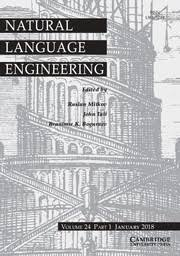
\includegraphics[width=.2\textwidth]{figures/nle-journal}
%	
\includegraphics[width=.63\textwidth]{figures/cambridge-core}
%\end{center}
%
%\textbf{\LARGE \alert{\url{goo.gl/A76NGX}}}
%	
%	
%\end{frame}


\begin{frame}{\alert{\textbf{Thank you! Questions?}} }

  \animategraphics[loop,autoplay,width=\linewidth]{2}{figures/he}{1}{4}

%
\includegraphics[width=0.25\textwidth]{figures/dfg} 
\includegraphics[width=0.15\textwidth]{figures/daad}

\end{frame}


